Avtomatska stružnica je stružnica, kjer so vsi 
gibi, kot na primer vključevanje glavnega vretena 
in podajalnih gibanj, sprememba števila vrtljajev 
glavnega vretena in podajalnih hitrosti, vpenjanje 
obdelovanca, vključevanje dodatnih naprav in drugo, 
v celoti avtomatizirani. Ob spremembi oblike 
obdelovanca je potrebno dolgotrajno nastavljanje krmiljenja.
Ko je to urejeno, pa delavec samo nadzoruje delovanje 
in občasno izmeri kose ter vloži novo palico materiala 
v podajalec.

Na avtomatskih stružnicah preprosto obdelujemo paličast
material, ki ga dovajamo v stroj skozi posebno vodilno 
cev, ki je v sredini glavnega vretena.

Material lahko tudi dovajamo v kosih preko dodajne 
naprave. Če so obdelovanci večji in 
nerodnih oblik, je njihovo delovanje lahko zelo težavno
in jih zato vpnemo ročno. Seveda pa v takem primeru 
ne moremo več govoriti o avtomatu, temveč o 
polavtomatskem stroju.

\noindent Avtomatske stružnice delimo na:
\begin{itemize}
    \item Eno-vretenske
    \item Več-vretenske
\end{itemize}

Spodaj so obe vrste avtomatskih stružnic. Levo, na sliki \ref{eno_vretenska_struznica}
je prikazana eno-vretenska stružnica, desno, na sliki \ref{vec_vretenska_struznica} 
pa je prikazana več-vretenska stružnica.

\begin{multicols}{2}
    \begin{figure}[H]
        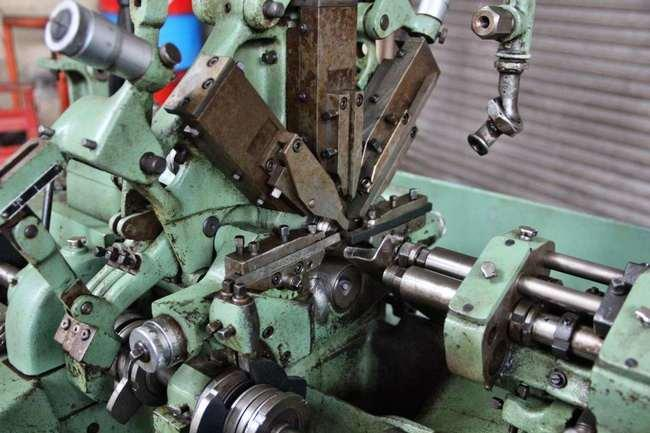
\includegraphics[width=\linewidth]{eno_vretenski_avtomat.jpg}
        \caption{Eno-vretenska stružnica
            \cite{eno_vretenska_struznica}}
        \label{eno_vretenska_struznica}
    \end{figure}

    \columnbreak

    \begin{figure}[H]
        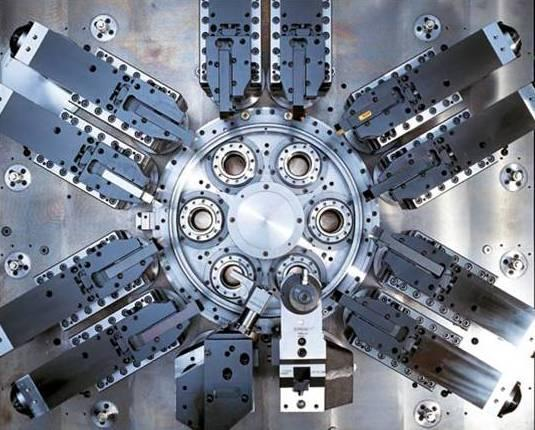
\includegraphics[width=\linewidth]{vec_vretenska_struznica.jpg}
        \caption{Več-vretenska stružnica
            \cite{vec_vretenska_struznica}}
        \label{vec_vretenska_struznica}
    \end{figure}
\end{multicols}